O \emph{LabInstru Web}, nome dado à plataforma desenvolvida no escopo deste trabalho de conclusão de curso, é o resultado da implementação das funcionalidades identificadas e prototipadas nas etapas anteriores. Esta plataforma foi desenvolvida utilizando o \emph{framework} Web2py, banco de dados MySQL e tecnologias como JQuery e Bootstrap. A página inicial da aplicação encontra-se ilustrada na Figura \ref{fig:ap1}. A partir da página principal da aplicação, é possível aos seus usuários utilizarem as funcionalidades para autenticação no sistema, vide Figura \ref{fig:ap10}, bem como para recuperação de senha, vide Figura  \ref{fig:ap11}.



\begin{figure}[h!]
	\centering
	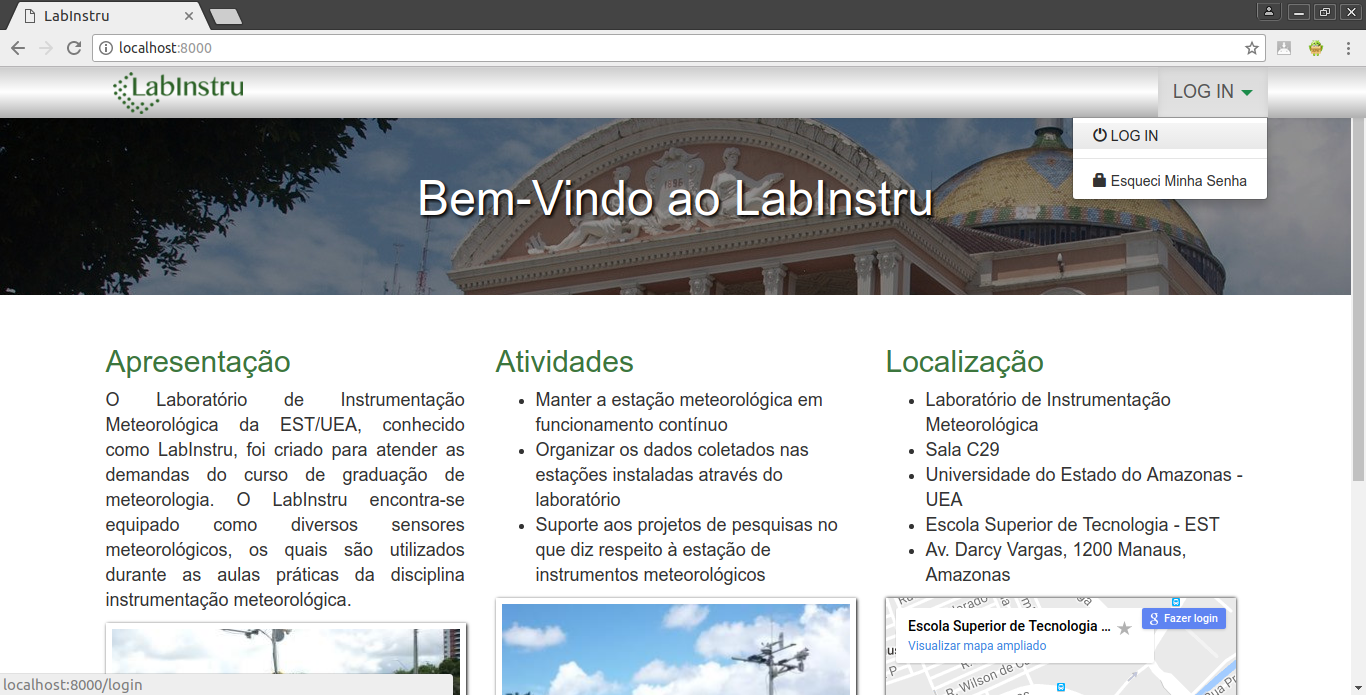
\includegraphics[width=0.9\textwidth]{./img/ap1.png}
	\caption{Página inicial da aplicação LabInstru Web. Fonte: Próprio autor.} \label{fig:ap1}
\end{figure}

\begin{figure}[h!]
	\centering
	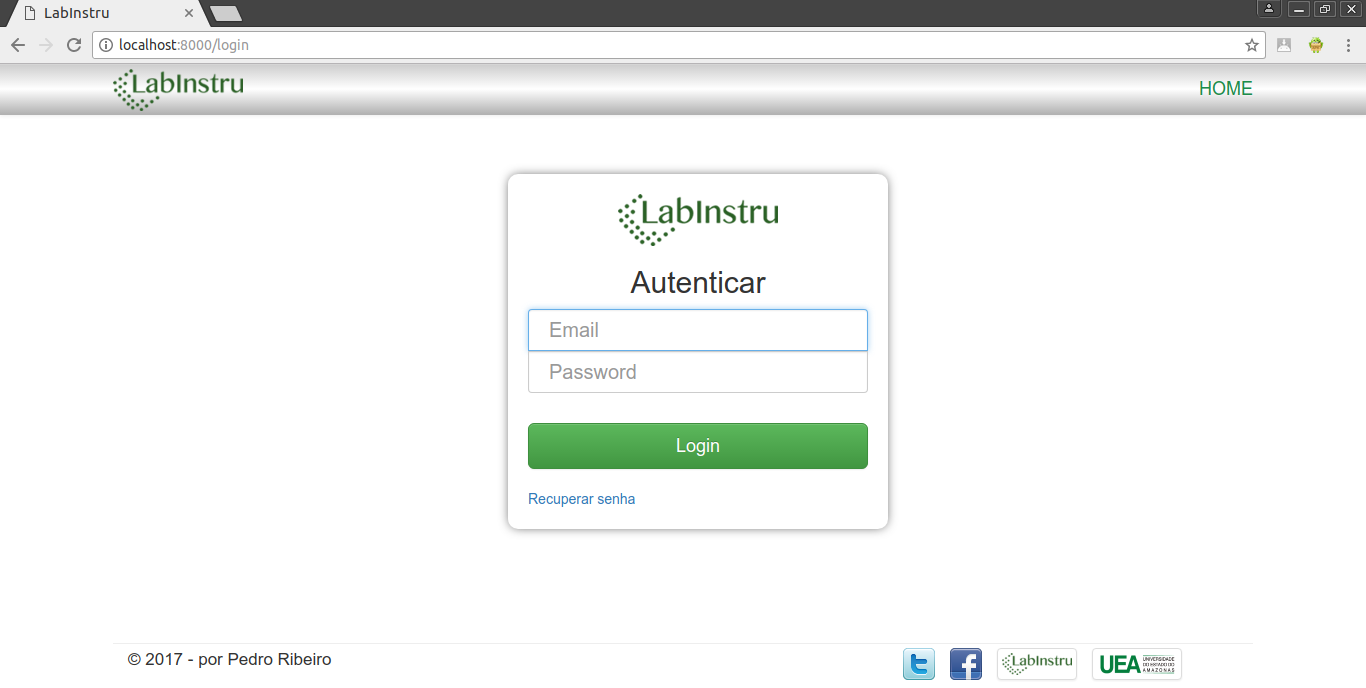
\includegraphics[width=0.9\textwidth]{./img/ap10.png}
	\caption{Formulário de autenticação do sistema. Fonte: Próprio autor.} \label{fig:ap10}
\end{figure}



\begin{figure}[h!]
	\centering
	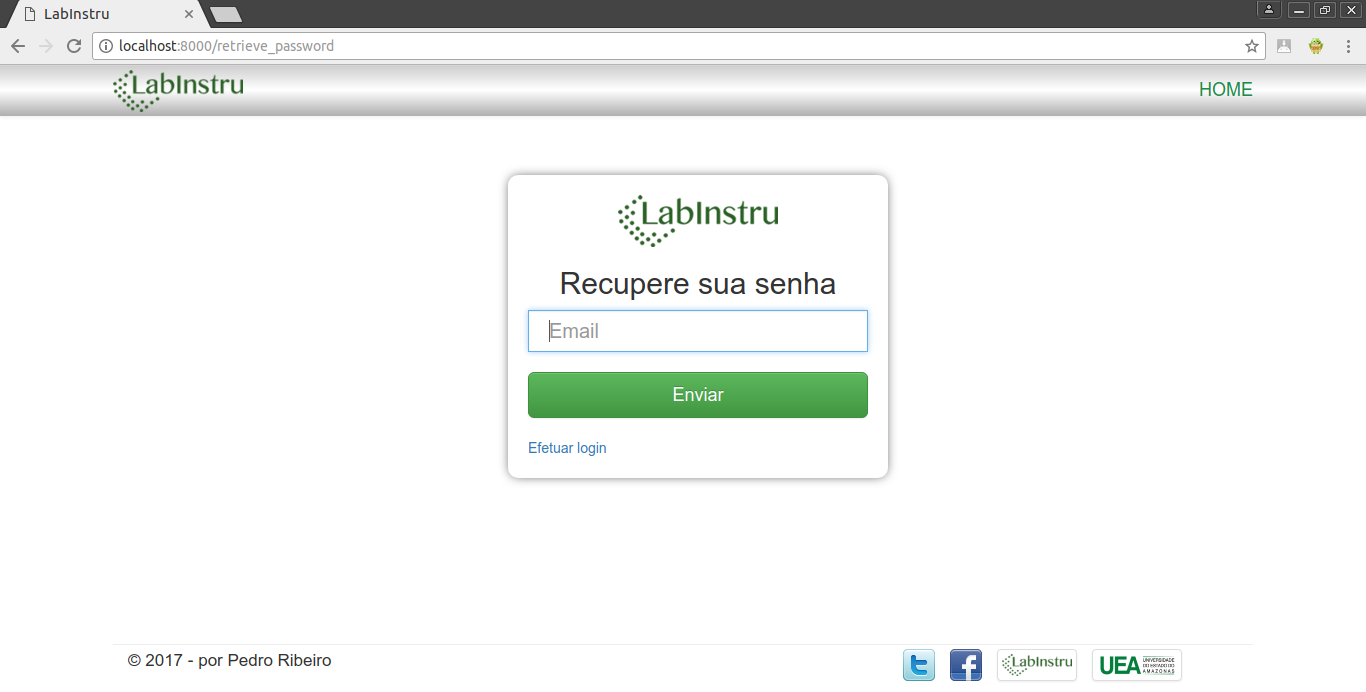
\includegraphics[width=0.9\textwidth]{./img/ap11.png}
	\caption{Formulário para recuperação de senha. Fonte: Próprio autor} \label{fig:ap11}
\end{figure}

A plataforma contempla dois perfis diferentes de acesso: um administrador, a ser desempenhado em termos práticos pela Profa. Maria Betânia Leal, responsável pelo LabInstru, e diversos usuários. O administrador, em especial, é o responsável por fornecer como entrada os dados advindos da estação meteorológica da EST para o LabInstru Web, conforme ilustrado na Figura \ref{fig:ap12}. A aplicação, após processar e persistir os dados advindos da estação, irá fornecer um sumário a respeito do status desta inserção, sob a forma de um \emph{log}. Este \emph{log} exibe quantas medições possuía o arquivo fornecido como entrada, quantas foram corretamente persistidas e quantas resultaram em falha. Um exemplo deste \emph{log} produzido pela aplicação é mostrado na Figura \ref{fig:ap13}.

\begin{figure}[h!]
	\centering
	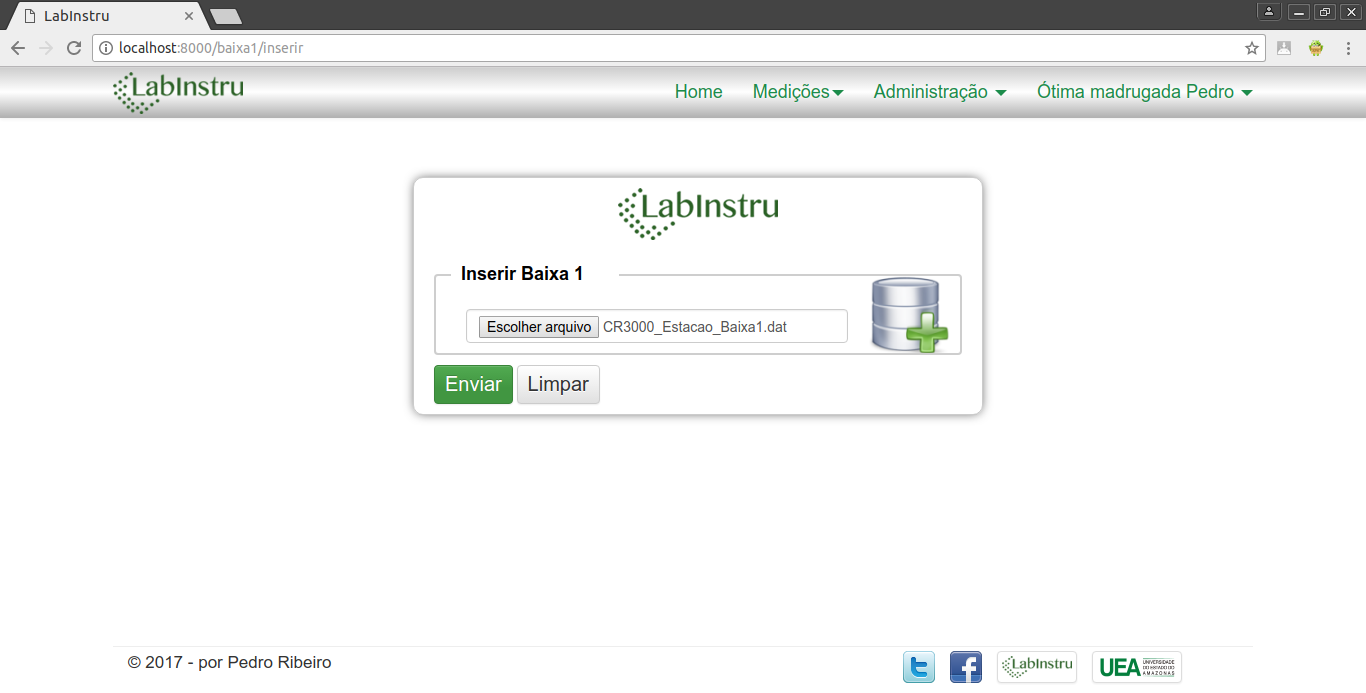
\includegraphics[width=0.9\textwidth]{./img/ap12.png}
	\caption{Página que disponibiliza o formulário para inserção de medições. Fonte: Próprio autor} \label{fig:ap12}
\end{figure}

\begin{figure}[h!]
	\centering
	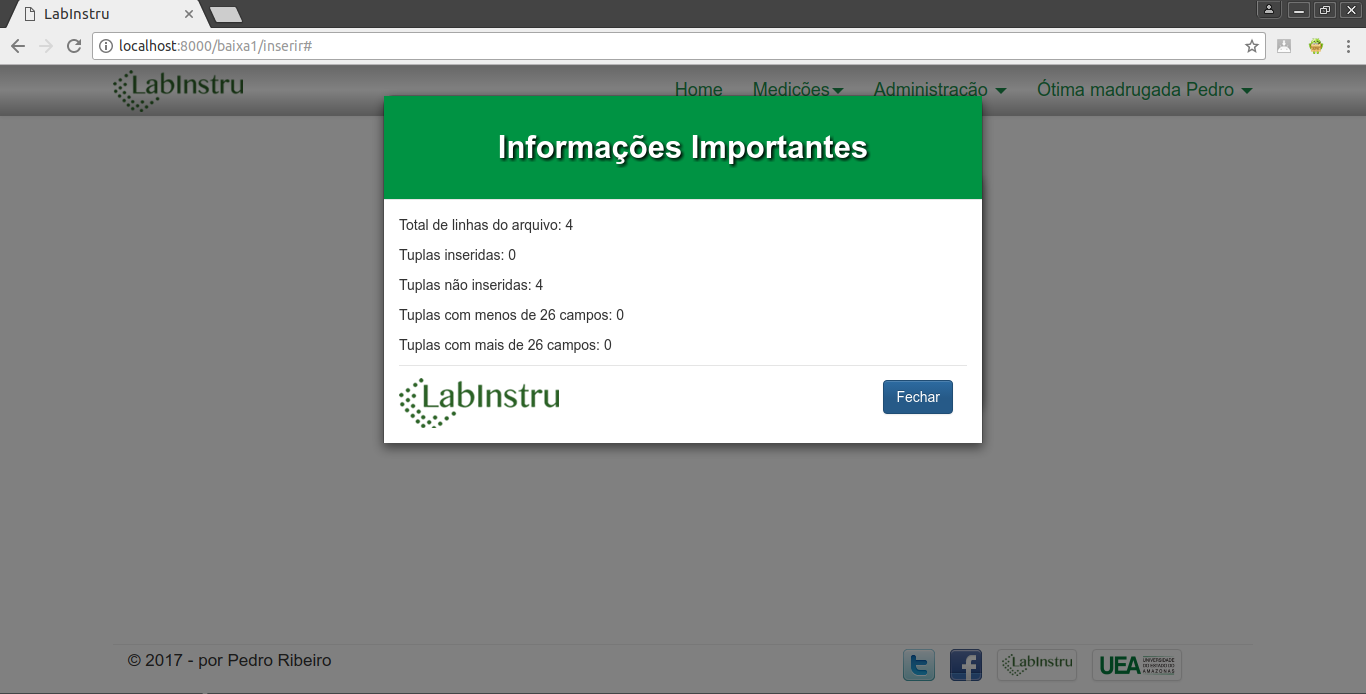
\includegraphics[width=0.9\textwidth]{./img/ap13.png}
	\caption{Exemplo de \emph{log} informando o resultado de uma inserção de medições. Fonte: Próprio autor} \label{fig:ap13}
\end{figure}



O administrador também fica responsável por cadastrar usuários, vide Figura \ref{fig:ap4}, que podem ser alunos de graduação e pós-graduação, outros pesquisadores, docentes, etc. Cabe também ao administrador da aplicação, por meio de uma listagem de usuários disponibilizada pela aplicação, realizar o gerenciamento dos usuários cadastrados na aplicação, conforme ilustrado na Figura \ref{fig:ap14}.

\begin{figure}[h!]
	\centering
	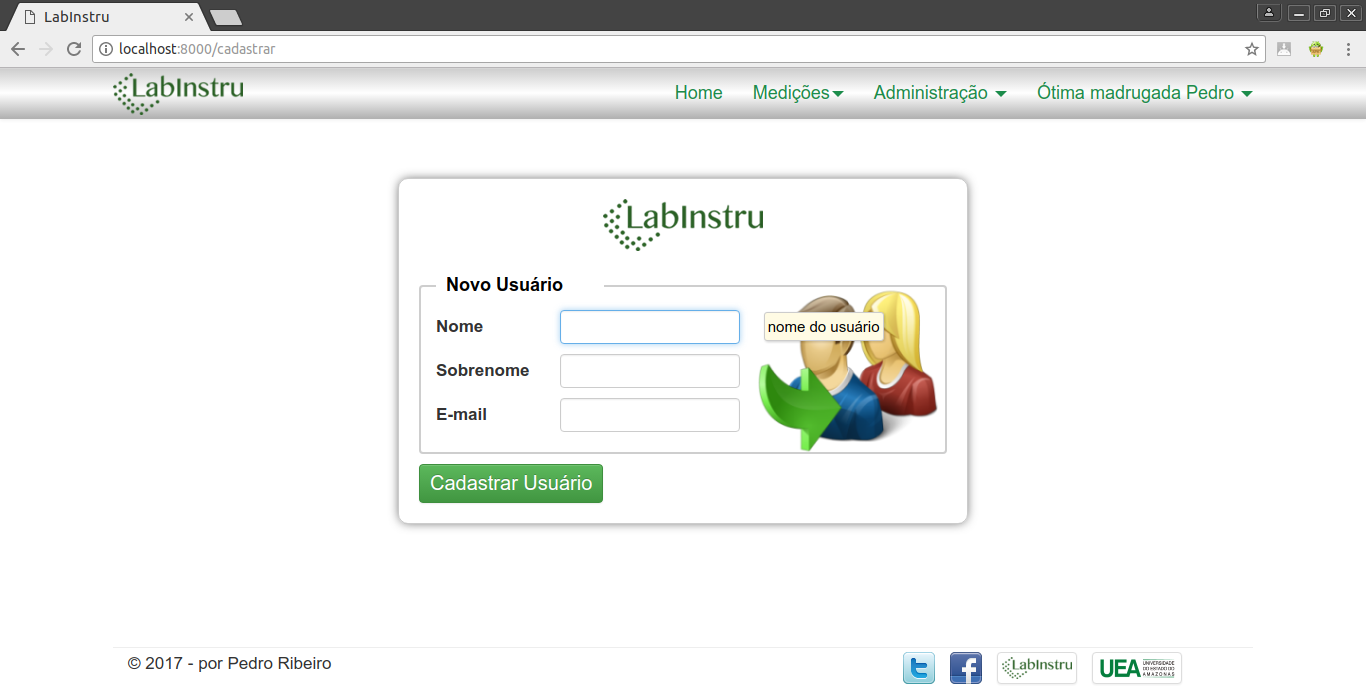
\includegraphics[width=0.9\textwidth]{./img/ap4.png}
	\caption{Página de cadastrado de usuário na plataforma LabInstru Web. Fonte: Próprio autor.} \label{fig:ap4}
\end{figure}

\begin{figure}[h!]
	\centering
	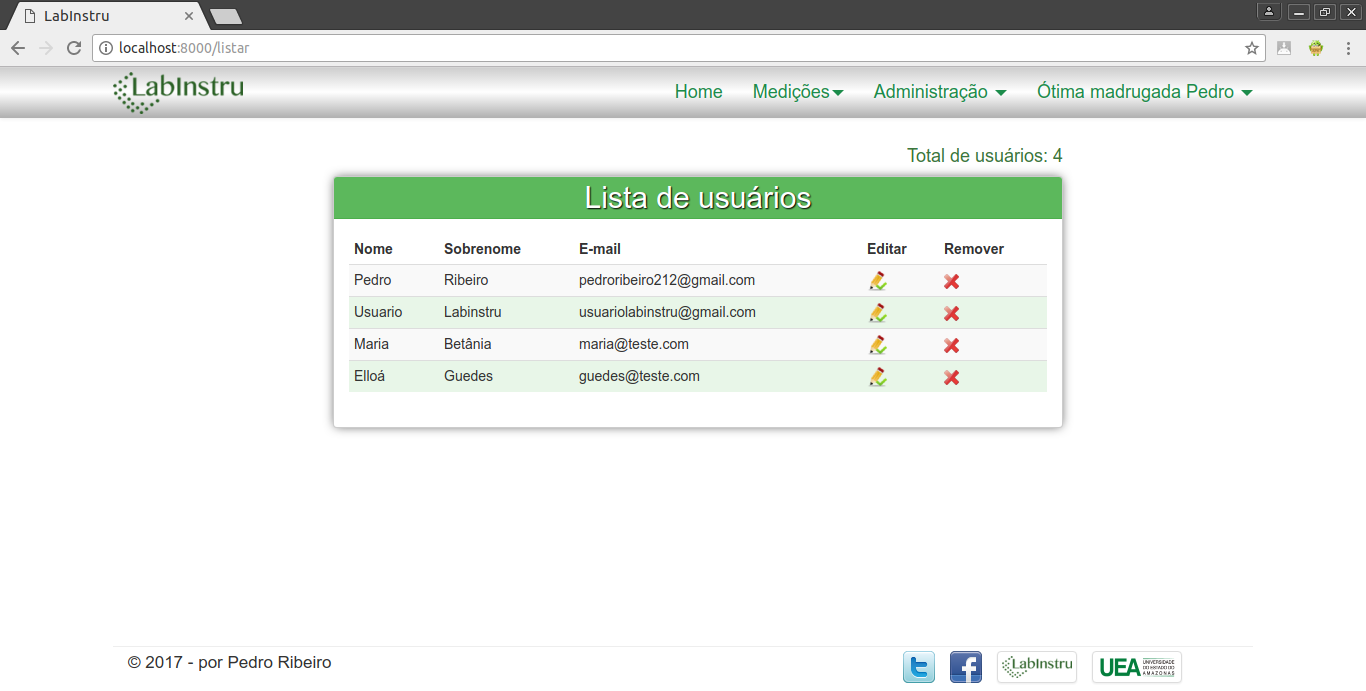
\includegraphics[width=0.9\textwidth]{./img/ap14.png}
	\caption{Lista de usuários cadastrados na aplicação. Fonte: Próprio autor.} \label{fig:ap14}
\end{figure}

Um menu superior, mostrado na Figura \ref{fig:ap1}, permite a autenticação dos usuários e também mostra as principais funcionalidades disponíveis na plataforma após realizada autenticação no sistema. Este menu é renderizado conforme o perfil do usuário. Por exemplo, o menu mostrado ao administrador dispõe da funcionalidade de apagar medições, funcionalidade não disponível no menu mostrado a um usuário. Os menus correspondentes aos diferentes perfis de usuário são ilustrados na Figura \ref{fig:ap8}. Ressalta-se que, independentemente do tipo do perfil de usuário, as principais funcionalidades da plataforma só poderão ser acessadas mediante prévia autenticação na plataforma via login e senha.

\todo{Nova versão da figura, refletindo o novo menu}
\begin{figure}[h!]
	\centering
	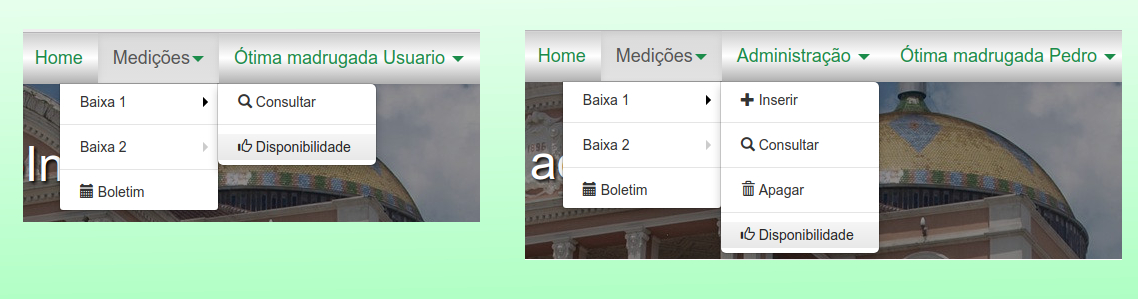
\includegraphics[width=0.9\textwidth]{./img/ap8.png}
	\caption{Exemplos dos menus para diferentes perfis de usuário. Fonte: Próprio autor.} \label{fig:ap8}
\end{figure}

As funcionalidades que permitem a mudança de senha e alteração de seus dados cadastrais são comuns aos dois perfis de usuários. Para ter acesso as mesmas, é necessário apenas que o usuário ou administrador encontre-se autenticado na aplicação. As Figuras \ref{fig:ap5} e \ref{fig:ap6} ilustram, respectivamente, os formulários para mudança de senha e alteração dos dados cadastrais de um determinado usuário (perfil).

\begin{figure}[h!]
	\centering
	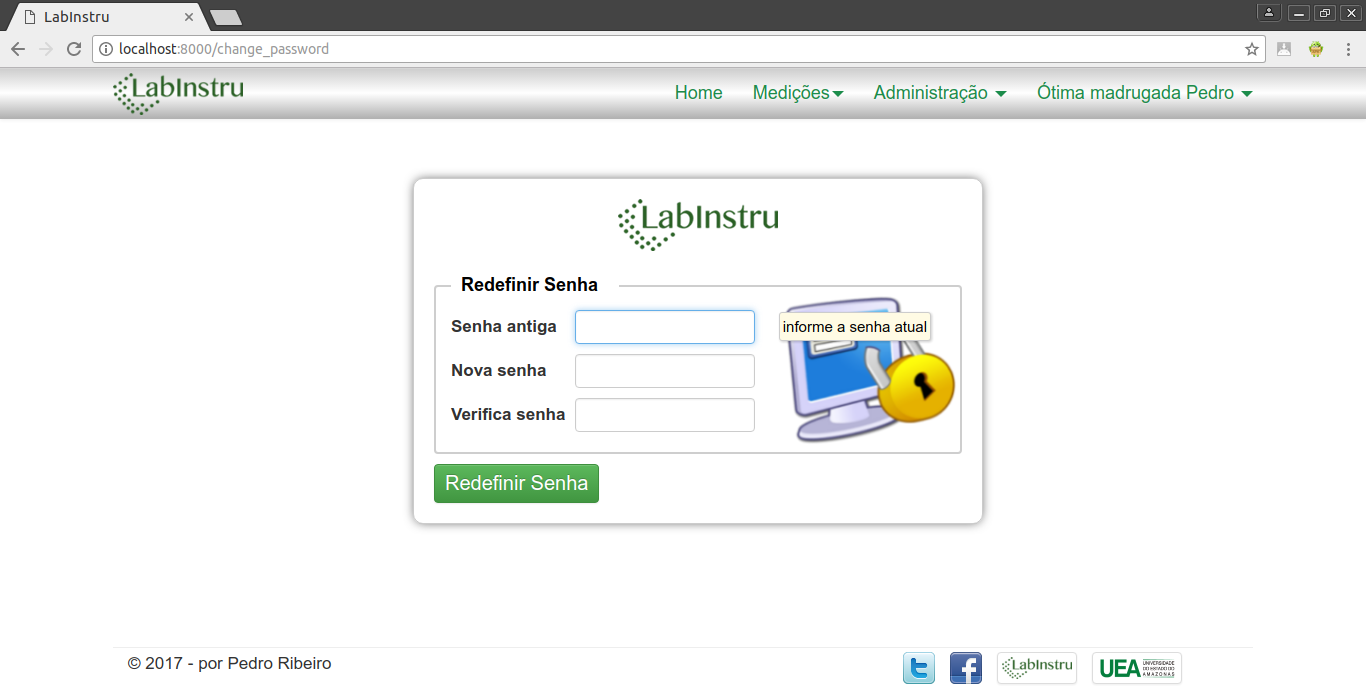
\includegraphics[width=0.9\textwidth]{./img/ap5.png}
	\caption{Formulário para troca de senha. Fonte: Próprio autor.} \label{fig:ap5}
\end{figure}

\begin{figure}[h!]
	\centering
	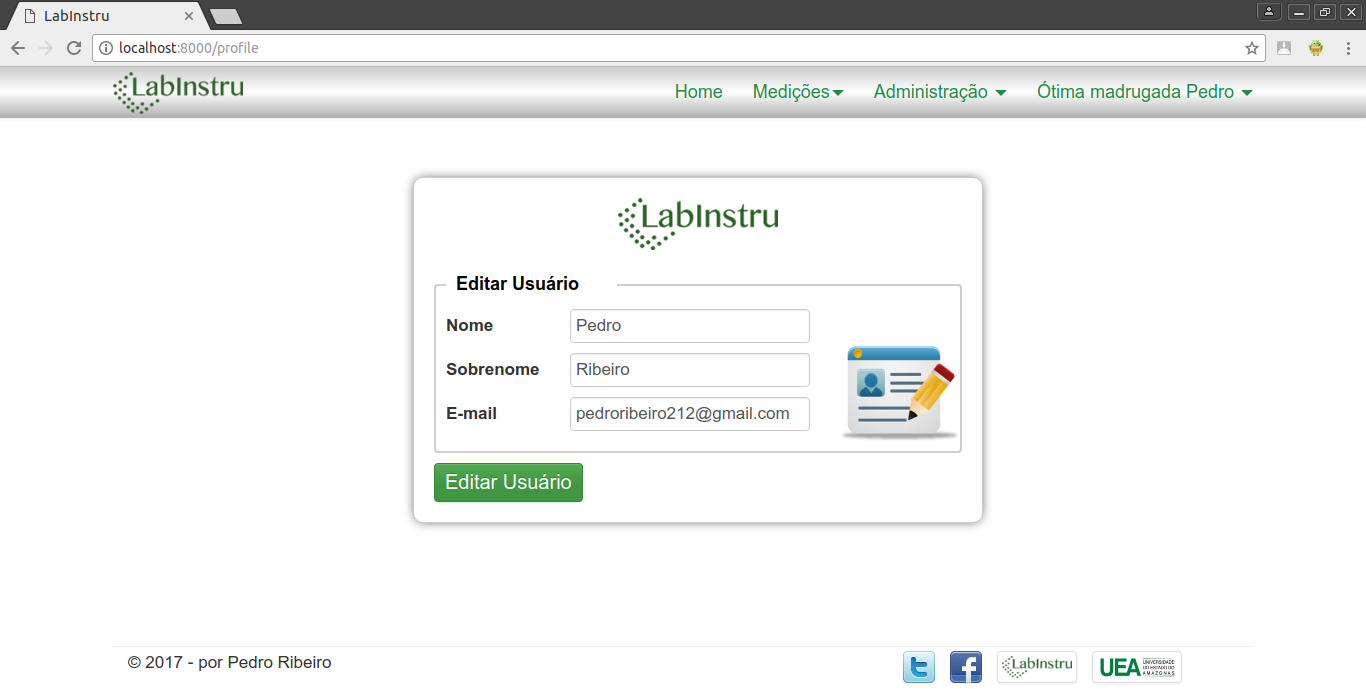
\includegraphics[width=0.9\textwidth]{./img/ap6.png}
	\caption{Página referente a edição de usuário. Fonte: Próprio autor.} \label{fig:ap6}
\end{figure}


Os usuários da plataforma \emph{LabInstru Web} acessam os dados da estação meteorológica da EST por meio de consultas, nas quais fornecem datas iniciais e finais e escolhem as variáveis de interesse, conforme ilustrado na Figura \ref{fig:ap3}. Considerou-se como uma restrição essencial para garantir a integridade e a confiabilidade dos dados que apenas o administrador seria responsável por cadastrá-los.

\todo{Atualizar esta figura}
\begin{figure}[h!]
	\centering
	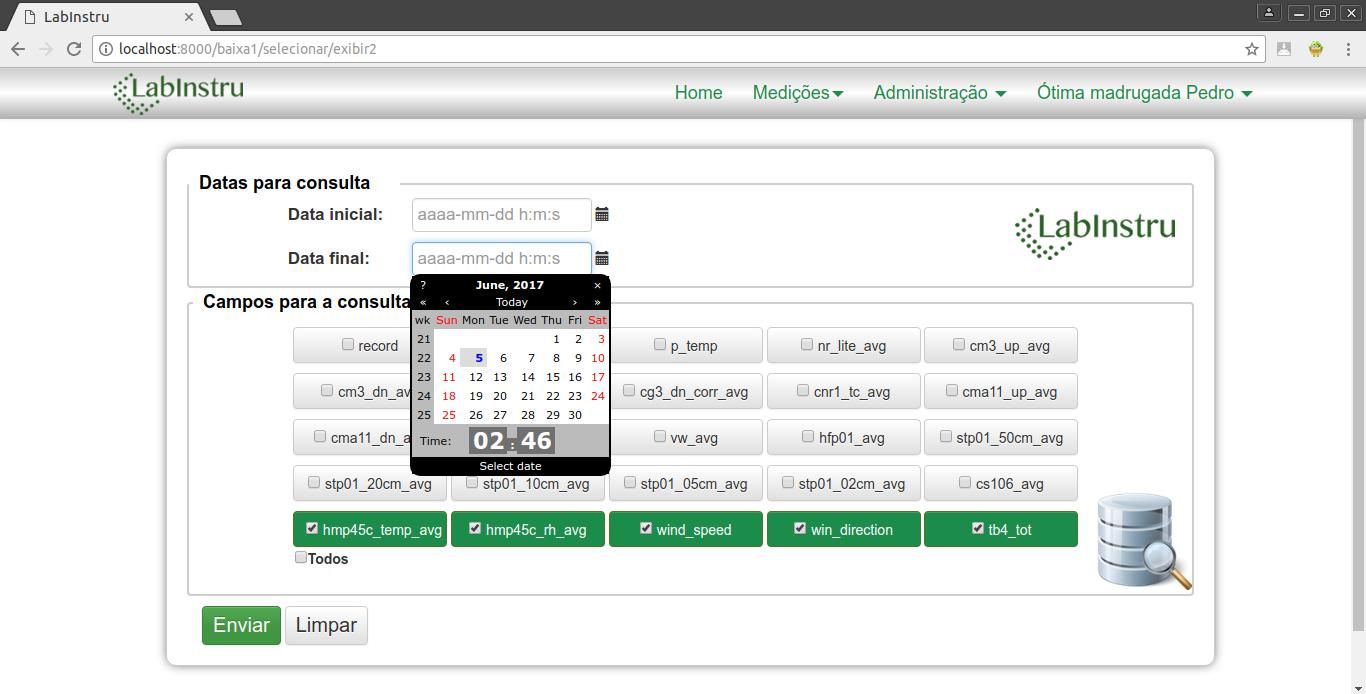
\includegraphics[width=0.9\textwidth]{./img/ap3.png}
	\caption{Página responsável por realizar as consultas. Fonte: Próprio Autor} \label{fig:ap3}
\end{figure}

Os resultados de uma consulta são exibidos em uma página apropriada, onde há opções para exportação dos mesmos nos formatos CSV, HTML, JSON, TSV e XML, conforme ilustra a Figura \ref{fig:ap7}.

\begin{figure}[h!]
	\centering
	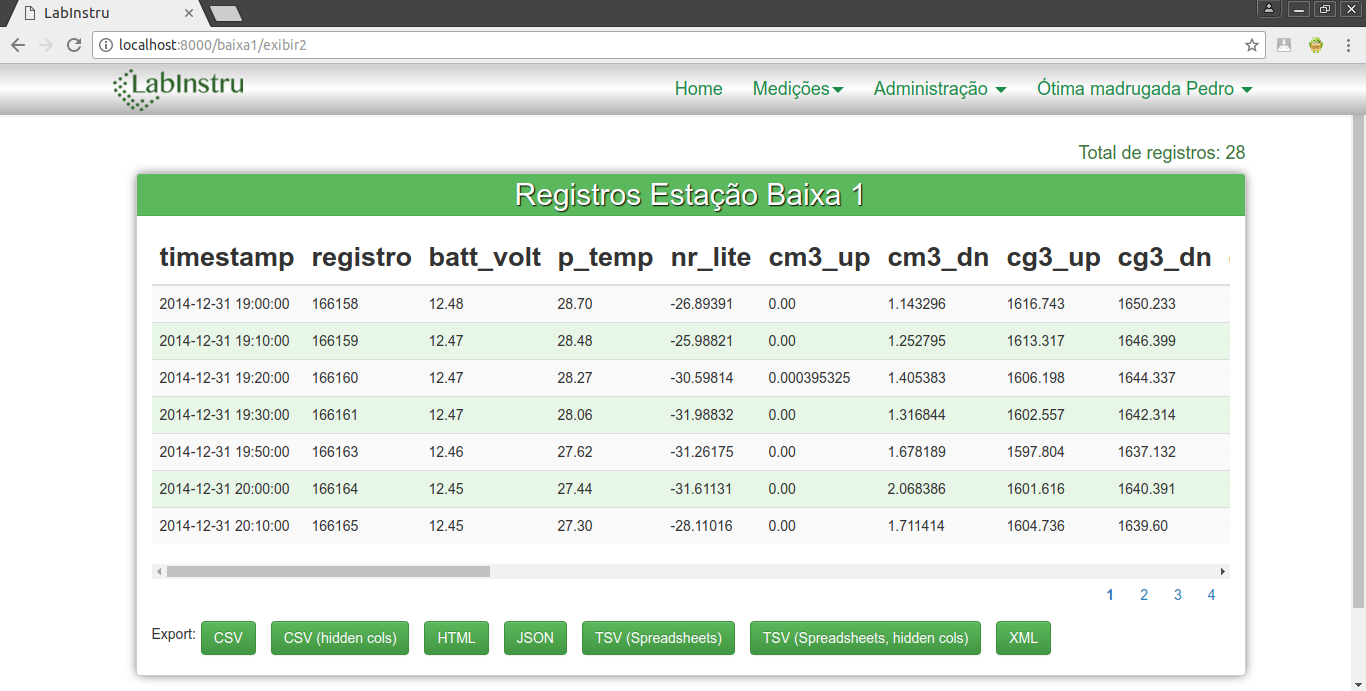
\includegraphics[width=0.9\textwidth]{./img/ap7.png}
	\caption{Página responsável por exibir o resultado de uma consulta. Fonte: Próprio Autor} \label{fig:ap7}
\end{figure}
